\documentclass[a4paper, 12pt]{article}
\usepackage{amsmath}
\usepackage{url}
\usepackage{graphicx}
\usepackage{listings}
\usepackage[hidelinks]{hyperref}
%\usepackage{hyperref}
\usepackage{cite}
\usepackage{color}
\usepackage{setspace}
%\usepackage[english]{babel}
\usepackage{minted}

\doublespacing
\definecolor{codegreen}{rgb}{0,0.6,0}
\definecolor{codegray}{rgb}{0.5,0.5,0.5}
\definecolor{codepurple}{rgb}{0.58,0,0.82}
\definecolor{backcolour}{rgb}{0.95,0.95,0.92}

\lstdefinestyle{mystyle}{
    backgroundcolor=\color{backcolour},   
    commentstyle=\color{codegreen},
    keywordstyle=\color{magenta},
    numberstyle=\tiny\color{codegray},
    stringstyle=\color{codepurple},
    basicstyle=\footnotesize,
    breakatwhitespace=false,         
    breaklines=true,                 
    captionpos=b,                    
    keepspaces=true,                 
    numbers=left,                    
    numbersep=5pt,                  
    showspaces=false,                
    showstringspaces=false,
    showtabs=false,                  
    tabsize=1
}

\lstset{style=mystyle}

\title{Extended Essay. Mathematics. \\ RSA: Encrypting, Decrypting, Hacking.}
%\date{06-12-2018}
\date{}
%\author{Sagindyk Urazayev}

\begin{document}

\pagenumbering{gobble}

\maketitle

%\begin{center}
%RSA: Encrypting, Decrypting, Hacking.\\
%\end{center}

\begin{flushleft}
\begin{figure}[b]
  Session: May 2018\\
%  School number: 007055\\
%  Student number: 0004\\
  Word count: 3975\\
\end{figure}
\end{flushleft}

\newpage

\pagenumbering{roman}

\tableofcontents
\newpage
\listoffigures
\listoftables
\lstlistoflistings

\newpage
\pagenumbering{arabic}

\begin{figure}[h!]
  \begin{center}
    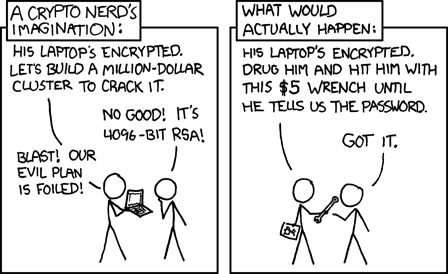
\includegraphics[width=0.6\textwidth]{xkcd_security.png}
    \caption{"Security" webcomic by Randall Munroe. Used with permission.\cite{xkcd}}
    \label{fig:xkcd}
    \end{center}
  \end{figure}

\begin{abstract}
\label{sec:abstract}

By starting this Extended Essay with a lovely webcomic by Randall Munroe, one can guess that the ``4096-BIT RSA'' sounds like it is tough to crack.
However, what is "RSA" and how does it work that even a "MILLION-DOLLAR CLUSTER" is not enough to crack it?\\
The research question of this Extended Essay is - ``Does RSA provide secure data transmission and confidential certificate signatures?''\\

This Extended Essay will explore the history of RSA
algorithm, the structure of the cryptographic technique, usage of it and ways to crack the algorithm.
For the sake of demonstration and proof, I have written several programs in C Language\cite{Clang} that can help us to understand the process "behind the curtains". After all these parts, at the end, we can conclude how RSA technique is secure.\\

Word Count : 133

\end{abstract}

\section{Introduction}
\label{sec:introduction}

First time when I heard about RSA technique, was during the ITGS class in IB course. In ITGS
Course Companion\cite{itgs} there is a
chapter about Security and Secret Key Encryptions. As an example, the author included two cases
of encryption: Symmetric Key Encryption or Single Key Encryption and Asymmetric key
encryption, more known as Public Key Encryption.\\

During the lesson, the fact that a message can be encrypted by one key and only a second key can
decrypt the message intrigued me. After that, I did some research on asymmetric encryptions,
particularly about RSA and other cryptographic technique based on it. I found that RSA is not only
used for messages encryption, but also for signing online certificates to prove one's identity. I
chose this topic for my Extended Essay because I believe the Mathematics in the algorithm is
simple and elegant; also, it is safe to say that RSA is used everywhere and the Internet trust relies
on this algorithm.\\

RSA encryption algorithm is essential if not the most critical security algorithm today, as nearly
every system in the world uses this asymmetric encryption technique to encrypt and decrypt data.
In this EE, I will be researching the methods of RSA: the way the algorithm works,
why it is considered secure, where and how it is used, mathematical proof with examples and ways
to break or brute-force the algorithm. 

\section{Historical background}
\label{bsec:historical_background}

Ever since people began to write down events or private information, there has been a need for
cryptography. Cryptography is a study of techniques of encrypting a text in such a manner that
outsiders to the code cannot understand the contents, but the desired reader can decrypt and read
the message in its original form. Just like for an early man and modern man, there always has been a
need for secrecy.\\

\subsection{Caesar Cypher}
\label{bsec:caesar_cypher}

First records of known cryptographic techniques go back to the times that were Before the
Common Era, in the times Julius Caesar. Caesar cypher or Caesar's code is one the first methods
of encrypting texts. It works in a way that there are a text and a key, where the key is an integer value.\\

The key shows a shift of letters in the document according to the Latin alphabet. For example, if
the key is two, then the first letter of the alphabet will become third, the second will become forth
and so on. During his lifetime, Julius Caesar mostly used three as a shift to protect messages of
military significance.\cite{singh}\\

\subsection{Enigma Machine}
\label{bsec:enigma_machine}

We can say for sure that the moment, when encryption was the tool of secretly transmitting data
so important and valuable that lives of thousands of people depended on how well that information
is transferred from one end to another, is World War II.\\

Enigma machine was the German
perfection of cryptography and engineering, the device so small and so complex, that it produced
code, which was considered as impossible to crack. However, during the war, a brilliant
mathematician and cryptographer Alan Turing found a flaw in Enigma Machine and was able to
build the first computer to exploit the system's vulnerability\cite{enigma}.\\

\subsection{Flaw in Symmetric Cryptography}
\label{bsec:flaw}

All existing algorithms had one most significant vulnerability in all of them- both ends should have
known the key or secret passphrase, which is used to encrypt and decrypt messages. In the example
with Enigma machine, German radio operators had a book with Enigma codes for the next month,
and it was a massive risk if hostile troops possess the codes. \\

\subsection{Whitfield Diffie and Martin Hellman}
\label{bsec:diffie}

The first attempt at solving the problem of symmetric algorithms goes back to a pair of
cryptologists: Whitfield Diffie and Martin Hellman. In the book by Simon
Singh \cite{singh}, there is a story about how these cryptographers came up with the idea of a public-key
encryption: “I walked downstairs to get a Coke, and almost forgot about the idea. I remembered
that I'd been thinking about something interesting, but couldn't quite recall what it was. Then it
came back in a real adrenaline rush of excitement. I was aware for the first time in my work on
cryptography of having discovered something really valuable.”\\

They have discovered a revolutionary type of cyphering – asymmetric cryptography. This means that it solved the problem of
single key encryption, where encoder and decoder needed to know the passphrase. Unfortunately, they did not find a one-way function for
solving the problem, they have published the concept in 1976 and left it open.\\

\subsection{Rivest, Shamir, and Adleman}
\label{bsec:rsa}

The paper released by Whitfield Diffie and Martin Hellman showed that there was a solution for
the problem of symmetric encryption in the form of a one-way function. Another trio of researchers
made the actual discovery and proof: Ron Rivest, Adi Shamir, and Leonard Adleman. Rivest,
Shamir, and Adleman were a perfect team, as Rivest was a computer scientist, who was tracking
all the latest scientific papers and with an ability to implement something new in new places.
Shamir is also a computer scientist with a lightning intellect and ability to directly focus on the
core of the problem. Adleman was a mathematician with broad knowledge and patience, so during
the research, he was finding flaws in the works of Rivest and Shamir, and ensured that
cryptographers did not follow a false lead.\cite{singh}\\

A year later Ron Rivest with the help of Adi Shamir
and Leonard Adleman has made a breakthrough by finding the desired one-way function, thus
solving the problem of symmetric encryptions. In 1977, the trio published a full paper
about the new asymmetric encryption technique, which was named after its creators- R.S.A.\cite{rsapaper}\\

\section{The Usage of RSA}
\label{sec:usage}

As an algorithm and cryptographic technique, RSA is brilliant without a doubt. It is safe to say
that RSA and its versions are used everywhere in our digital world. It is crucial for modern
cryptography techniques to be sophisticated for computers to brute-force but not too complicated
and inefficient for computers to encrypt and decrypt data. RSA is located right in the middle, as
the operations performed in part \ref{sec:math} do not need a lot of computational power but to attack it requires a lot of it.
For more information please refer to part \ref{sec:security}\\

To demonstrate the work and the functionalities of the algorithm, three types of cryptography techniques will be displayed:
single key encryption, assymetric encryption and certificate signatures.\\

\subsection{Symmetric Encryption}
\label{bsec:symmetry}

This type of encrypting and decrypting algorithms is the oldest way to cypher data. It works with
one key, one text and two ends. On the first end, there is an encoder, who cyphers the text with a
known key and then sends the encrypted data to the other end, decoder, who later decrypts text
with the same key. The example with Blowfish\cite{blowfish} algorithm with key
“jeopardize” can be seen below in Figure \ref{fig:symmetric}.

\begin{figure}[ht]
  \begin{center}
    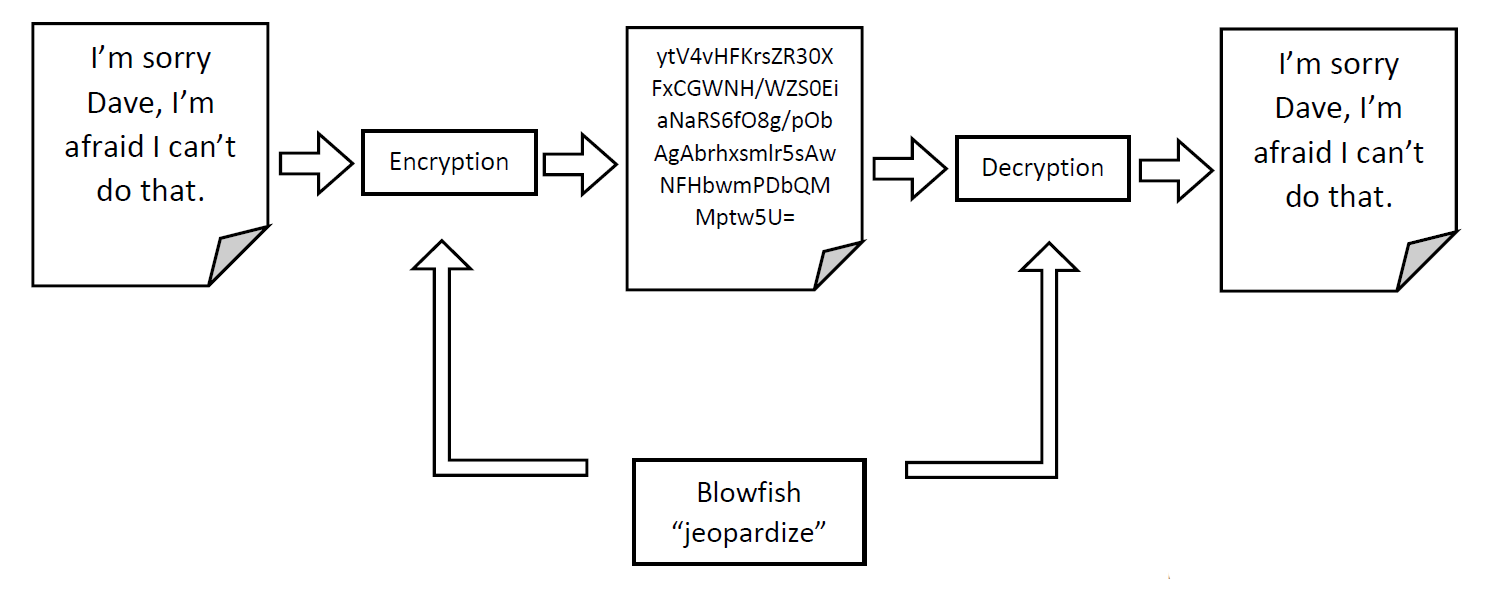
\includegraphics[width=\textwidth]{symmetric.png}1
    \caption{Example of Symmetric Encryption}
    \label{fig:symmetric}
    \end{center}
  \end{figure}

The downside is that both ends of the transmission should know the shared key. In the scenario where
people have met and shared the encryption key in real life, there is no danger that someone can
steal the shared key and decrypt transmissions. The problem arises when we have a scenario where
parties on both ends never talked with each other and are located on distinct physical locations.
Both ends want to transmit data securely, so the eavesdropper in the
middle will not understand the contents of the transmitted information.\\

In this scenario, it is
impossible to transmit data securely, because to decrypt text messages, both ends should know
the same key. Before the conversation, one end should send the key to the other end; however,
the eavesdropper will be able to "sniff" the key and will be able to understand all further encrypted
transmissions, thus compromising all further interactions.\\

\subsection{Asymmetric Encryption}
\label{bsec:asymmetric}

Asymmetric encryption relies on two distinct keys, where one is
used for encrypting data and the second one is for decrypting data that was decoded by its unique pair.
Keys for encrypting and decrypting are called public and private, respectively. There are two ways
of using RSA: to send an encrypted message to the decoder and signing certificates for
proving one's identity.\\

\subsubsection{Encrypting Messages}
\label{bbsec:encryption}

Every user has a pair of connected keys: a public key and private key. The public key is available
to everyone while the private key should be kept private to the owner of the unique pair
of keys. It is a preferred way of encryption; because both ends do not need to exchange the secret
key, they would already know the required part of the pair to transmit messages securely.
Continuing from part \ref{bsec:asymmetric}, this is widely used for secure data transmissions.\\

Imagine a scenario with three
users: Hal, Dave, and Eavesdropper. If Hal wants to send a message to Dave, Hal should use Dave's
public key and encrypt the desired message, later Hal sends an encrypted message to Dave. As
eavesdropper is sitting in the middle of Hal and Dave's transmission line, he can intercept the
transmitted data, make a copy of it and send it forward to Dave, thus having a copy of the letter.
Now, Dave and Eavesdropper have the encrypted message from Hal. Dave, using the private key
that is available only to him, can decrypt the message from Hal and read the contents. Fortunately,
the eavesdropper has access only to Dave's public key and not to his private key, so he is not able to read
message's contents.\\

The transmission is shown in Figure \ref{fig:asymmetric}.

\begin{figure}[h!]
  \begin{center}
    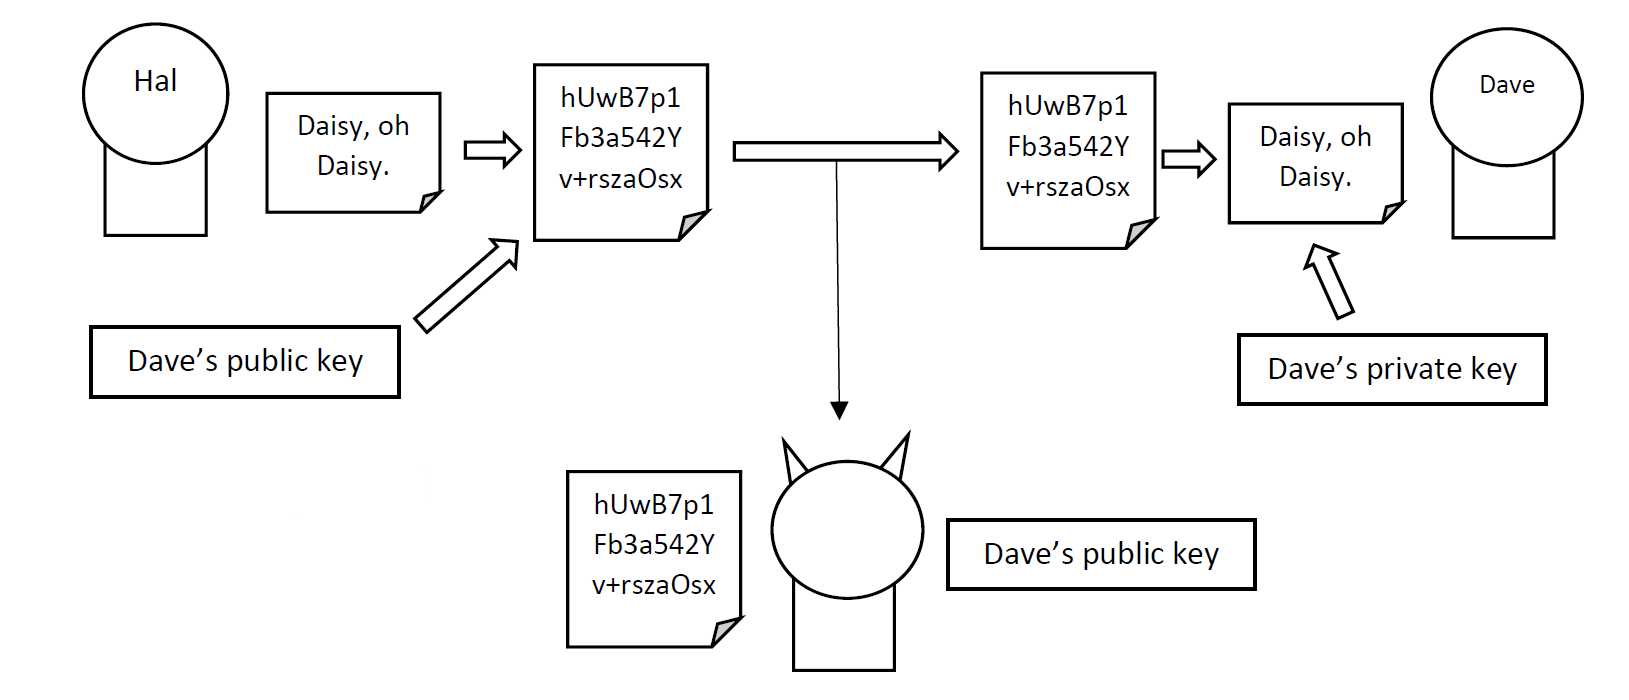
\includegraphics[width=\textwidth]{asymmetric.png}
    \caption{Example of Asymmetric Encryption}
    \label{fig:asymmetric}
    \end{center}
  \end{figure}

\subsubsection{Signing Certificates}
\label{bbsec:signing}

RSA encryption and decryption works in both ways, so a
message can be encrypted by a public key and decrypted by the private key and vice versa.\\

Imagine a scenario, when Hal wants to send an email to Stanley. The problem is that Hal is not sure
if Stanley is indeed Stanley and not a thief who stole Stanley's identity. To resolve the issue, RSA
technique should be used. \\

Hal and Stanley have a common friend - Dave. Dave can prove Stanley's identity by signing Stanley's
public key with his private key. Later, Hal can decrypt Stanley's public key with Dave's public key.
With this, Hal would be confident about Stanley's identity.\\

This whole process is based on trust. If Person A will sign a key of an untrusted entity, Person B, all other parties
would lose trust in Person A as he compromised secure network by signing unknown public key.\\

\section{Mathematical Foundation of RSA}
\label{sec:math}

The mathematics involved in keys generation and RSA algorithm require knowledge on modular
arithmetic, greatest common divisors, Euler's totient function, prime number theorem. In order to
make the calculations understandable and not hard to follow, I will make an introduction to
required theorems and formulas before the RSA steps.\\

\subsection{Modular Arithmetic and Congruence}
\label{bsec:mod}

In mathematics, the modulus is the operation to get the remainder when diving one number by
another. For example, if we want to find modulus of $31$ to $9$, we use the notation: $31\bmod9$, this
means that we divide $31$ by $9$ and take out only the remainder, in this case, it is going to be $4$.
Congruence means that if two numbers $b$ and $c$ have the property that their difference $b - c$ is
integrally divisible by a number $m$, so that $(b - c)/m$ is an integer, then $b$ and $c$ are said to be
"congruent modulo $m$", where $m$ is called the modulus. The notation as follows:

\begin{equation*}
  b \equiv c \text{ } (\bmod m)\\
  \end{equation*}

\subsection{Euler's Totient Function}
\label{bsec:euler}

The Euler's totient function $\varphi(n)$ is defined as a function that returns a number of positive integers
$<n$ that are relatively coprime to $n$, this means that they are not sharing any common factor. For
example, the totatives of $n = 9$ are $1, 2, 4, 5, 7 \text{ and } 8$. So that $\varphi(9) = 6$. For prime number $p$, the
number of totatives will be $p - 1$, as no integers share same multiples with $p$, except $p$.\\

\subsection{Greatest Common Divisor}
\label{bsec:gcd}

Greatest common divisor, using the notation $gcd(a,b)=c$, means that $a$ and $b$ share some common
divisors and where $c$ is the largest divisor. For example: $gcd(24,9)=3$. If we have an
expression that $gcd(d,e)=1$, it means that d and e are coprime because they are both integrally
divisible only by one.\\

\section{RSA}
\label{sec:rsa}

There are five main steps to generate public and private keys and two steps for encryption and
decryption together. More detailed information about that in the next parts.

\subsection{Key Generation}
\label{bsec:key}

\begin{enumerate}
\item Generate two distinct primes $p$ and $q$
  \begin{itemize}
  \item Primes $p$ and $q$ are recommended to be from 100 digits to 200 digits long. Because
of security reasons, primes $p$ and $q$ should be chosen at random, be similar in
magnitude, but differ in digits number, so the factoring would be harder.
\item The factoring problem will be discussed in chapter 5.
  \end{itemize}
\item Find $n=p \times q$
  \begin{itemize}
  \item It is not difficult for computers to multiply values of $p$ and $q$, even if they are primes and big
in size, in terms of amount of bits.
\item During the encryption and decryption steps, $n$ would be used as a modulus for
public and private keys.
\item Usually, the key length is referred to the length of $n$. The bigger the key size is, then keys are considered more secure.
  \end{itemize}
\item Compute $\varphi(n) = \varphi(p) \times \varphiφ(q) = (p-1) \times (q-1)$.
  \begin{itemize}
    \item Referring to part \ref{sec:math}, we know how the Euler totient formula works and how it is
applicable for prime numbers.
\item This value should be kept private.
    \end{itemize}
  \item Choose $e$, so that $1 < e < \varphi(n)$ and $gcd(e), \varphi(n)) = 1$.
    \begin{itemize}
      \item $e$ is our public key component, which is public and should be coprime to Euler
totient function of $n$.
      \end{itemize}
  \item Determine $d$, as $d \times e \equiv 1 \bmod (\varphi(n))$.
    \begin{itemize}
    \item Referring to part \ref{sec:math}, this can be solved by knowing that
      \begin{equation*}
        d \times e \equiv k \varphi(n) + 1\\
        \end{equation*}
        All variables in the equation are positive integers.
      \end{itemize}
  \end{enumerate}

\subsection{Encryption and Decryption}
\label{bsec:ed}

After completing the necessary calculations, which are described in part 4.1, the large prime
numbers $p$, $q$, and totient value of $n$- $\varphi(n)$ should be deleted or not revealed to anyone except the
host, where keys were generated. We have two generated keys: a public key and private key. The
host should share his/her public key, so it is available to anyone and keep the private in secret. As
the RSA encryption method is described in part \ref{bsec:asymmetric}, we will continue now with the process of
encryption and decryption, later on, accompanied by two examples.\\

Let us return to the scenario with Dave and Hal in part \ref{bsec:asymmetric}. Hal wants to send Dave a message, so
he knows only Dave's public key. To encrypt the message and transmit it securely, Hal firstly
converts his message from plaintext to numerical values, for example, binary, octal, decimal, and
hexadecimal etc. Because of Dave's public key, Hal knows the public exponent $e$ and modulus $n$.
By using the encryption formula below

\begin{equation*}
  c = m^e \bmod n\\
  \end{equation*}

Where $m$ is converted text and $c$ is the encrypted message, Hal now has a uniquely encrypted
message and so can send it to Dave. On the other end of the communication line, Dave receives
the encrypted message $c$ and by knowing private exponent $d$ and modulus $n$ from his private key,
Dave and only Dave can decrypt the following message using the formula below.

\begin{equation*}
  m = c^d \bmod n\\
\end{equation*}

It can be seen that the formula for encryption and decryption are inverse, the only exceptions are
the public and private exponents, which are connected to each other, as only in right pairs,
encryption and decryption would take place. Thus, this is considered a one-way function, so
without knowing the public exponent and private exponent, at the time it is considered impossible
to brute-force private exponent. The reason for this will be explained in part \ref{sec:security}.\\

\subsection{Examples of RSA}
\label{bsec:example}

In this part I will include two RSA examples.\\

\subsubsection{First Example with Small Primes}
\label{bbsec:first}

For the first example, we will use small primes in the range from 2 to 20. For this part, I will make
some of the calculations by hand, after 4th step, I will use Wolfram Alpha to compute data.

\begin{enumerate}
\item We should choose our prime numbers $p$ and $q$. In this example, the values are
  \begin{equation*}
    p=11 \text{ and } q=13\\
  \end{equation*}
  \item In order to calculate modulus, I will multiply these two primes and the result will be
    the modulus $n$
    \begin{equation*}
      n=p \times q=11 \times 13=143
    \end{equation*}
    \item Using Euler's totient function, we can find the number of integers that do not share any
      common multiples with modulus $n$.
      \begin{equation*}
        \varphi(n)=\varphi(p) \times \varphi(q)=(p-1) \times (q-1)=(11-1) \times (13-1)=10 \times 12=120\\
      \end{equation*}
      \item Choosing the right public exponential $e$ is very important because we want the encryption
process to be fast, for that, we should pick a secure and reasonably small value. For this
example, $e=7$

\item Now we should find the private exponent
  \begin{align*}
    d \times e &\equiv 1 \bmod(\varphi(n))\\
    d \times e \bmod(\varphi(n)) &\equiv 1 \bmod(\varphi(n)) =1\\
    d \times e = k \times \varphi(n) + 1\\
  \end{align*}
  Where k is some positive integer constant, so that $(k \times \varphi(n) + 1)/(e)$ is an integer
  \begin{equation*}
    d = \frac{k \times \varphi(n)+1}{e}\\
    \end{equation*}
\end{enumerate}

Substituting variables from our example, we will get that $d=103$.\\

Now, we have calculated public and private keys:

\begin{align*}
  \text{public key}&=(e,n)=(7,143)\\
  \text{private key}&=(d,n)=(103,143)\\
  \end{align*}

Now, let us try to encrypt some message and then decrypt it. In order to prove the work of RSA, I
will encrypt the message – "ATTACK AT DAWN".\\

Firstly, we need to convert the plaintext into numbers, so we can use the encryption and decryption
formula. Table \ref{table:simple} below presents the way we will convert the plaintext.

\begin{table}[h]
  \begin{center}
        \caption{Table on How Individual Characters Will be Converted into Digits}
    \begin{tabular}{c|c|c|c|c|c|c|c|c|c|c|c|c}
      A& B& C& D& E& F& G& H& I& J& K& L& M\\
      \hline
      01& 02& 03& 04& 05& 06& 07& 08& 09& 10& 11& 12& 13\\

      N& O& P& Q& R& S& T& U& V& W& X& Y& Z\\
      \hline                   
      14& 15& 16& 17& 18& 19& 20& 21& 22& 23& 24& 25& 26\\
    \end{tabular}
    \label{table:simple}
  \end{center}
  \end{table}


After converting each letter, we will get the following: 012020010311012004012314. We
consider that spaces between words are not convertible and we skip them. To encrypt the message
efficiently, we will encrypt each pair using our public key, where our public exponent is 7 and
modulus is 143. The following calculations have been completed by using Wolfram Alpha. I will
calculate only unique letters’ codes and then combine it to make an encrypted message. Notation
$Encrypt(N)$ will be used for simplicity, where $N$ is the number of a letter or a letter from Latin alphabet.
"$???$" will be used to represent a letter that cannot be converted from digits, according to the table above.

\begin{align*}
  &Encrypt(A)=&Encrypt(01)=01^7 \bmod 143=1 \bmod 143=01&=A\\
  &Encrypt(C)=&Encrypt(03)=03^7 \bmod 143=2187 \bmod 143=42&=???\\
  &Encrypt(D)=&Encrypt(04)=04^7 \bmod 143=16384 \bmod 143=82&=???\\
  &Encrypt(K)=&Encrypt(11)=11^7 \bmod 143=19487171 \bmod 143=132&=???\\
  &Encrypt(N)=&Encrypt(14)=14^7 \bmod 143=105413504 \bmod 143=53&=???\\
  &Encrypt(T)=&Encrypt(20)=20^7 \bmod 143=1280000000 \bmod 143=136&=???\\
  &Encrypt(W)=&Encrypt(23)=23^7 \bmod 143=3404825447 \bmod 143=23&=W\\
\end{align*}

The original message's code is 012020010311012004012314, will be encrypted to
0113613601421320113682012353, which obviously does not look like our initial input. This is
the encrypted message; it is non-readable and non-understandable to all users. Only the receiver
with the private key can decipher the message and find the initial content.\\

It is noticeable that encrypted version of A and W are the same. This can be viewed as a flaw in RSA, however,
the probability of this correspondence is very low and individual letters would not compromise the message's
initial contents.\\

As we have the private key with the private exponent, we can decipher the encrypted message and
calculate the content of the initial message. To do that so, the decryption formula will be used. Rising
numbers to power 103 will give us very big numbers. Calculations below include only the result,
for the extended calculations please refer to \ref{calc}. Function called $Decrypt(N)$ will be used
for simplicity to represent decryption process, where $N$ is an encrypted number that should be
deciphered with the appropriate private key.

\begin{align*}
  &Decrypt(01)=&01^{103} \bmod 143=01&=A\\
  &Decrypt(42)=&42^{103} \bmod 143=03&=C\\
  &Decrypt(82)=&82^{103} \bmod 143=04&=D\\
  &Decrypt(132)=&132^{103} \bmod 143=11&=K\\
  &Decrypt(53)=&53^{103} \bmod 143=14&=N\\
  &Decrypt(136)=&136^{103} \bmod 143=20&=T\\
  &Decrypt(23)=&23^{103} \bmod 143=23&=W\\
\end{align*}

After the decryption, we can rebuild the initial message- “ATTACK AT DAWN”.
RSA has proved its work with small values of $p$ and $q$, we can test RSA for bigger values.\\

\subsubsection{Second Example with Large Primes}
\label{bbsec:second}

In order to work with big primes, calculations by hand or Wolfram Alpha will become inefficient
and quite difficult. To demonstrate the work of RSA, I wrote a program in C. 
The program takes an input of modulo - $n$, public exponent - $e$, private exponent – $d$
and a message that needs to be encrypted. More detailed information about the code in Appendix\ref{big}.\\
The input message will be encoded in hexadecimal by using ASCII table. Using
the message’s representation in hexadecimal, the program will encrypt it using the public key, later
will make an attempt of reading the contents of the encrypted message and finally decrypting the
message using the private key. I wrote this program for this Extended Essay to demonstrate the
work of RSA encryption algorithm with big primes and proving the security of RSA later in section \ref{sec:security}.
The input and output of the program will be shown in boxes below. Calculations have been
made on a computer with specifications that can be found in Appendix \ref{specs}.\\

I have entered values 516311845790656153499716760847001433441357,\\ 65537 and
5617843187844953170308463622230283376298685 for modulo n, public exponent e, and private
exponent d, respectively. p and q values are unknown. We will encrypt message – “The cake is a
lie”. The executed program shows the hexadecimal version of our message and the encrypted
value of our message. When we try to read it, we get “c?SX?|ˆT??tv??”, which is not our
initial message. The encrypted value will be deciphered, using the private key. We will get our
initial message – “The cake is a lie.” Further details and examples can be found on my Github\cite{github}.\\

\section{Security of RSA}
\label{sec:security}

As mentioned above, RSA encryption algorithm is considered secure. The key
generation is not very expensive operation in terms of computer resources. For computers,
multiplication is a very easy task and they can do it easily. On the other hand, if we know n, to
find two prime numbers $p$ and $q$ is a tough challenge. There is a challenge, where people around
the world are trying to factor values of $n$, thus meaning finding initial prime $p$ and $q$.\cite{rsa}\\

RSA Factoring Challenge is a challenge by RSA Laboratories. They have calculated multiple n on
a computer with no network connection and all the hard are destroyed in order to keep $p$ and $q$ a
secret.\\

The factoring is a very big mathematical challenge because in general we will need to brute-force
all possible combination and find the correct match.\\

\subsection{Full Brute-Force}
\label{bsec:full}

Full brute-force algorithm will try all $p$ and $q$ number from 2 to n and will try to find a match. My
implementation of this algorithm can be found in Appendix \ref{fullbrute}. Generally, the algorithm runs two
nested loops, each with n steps. The performance can be described as $O(n^2)$, where $n^2$ is the
expected number of calculations required during the worst-case scenario.
This algorithm is very slow, for example, some $n$ with a value of
9237079 will require $9237079^2 = 85323628452241$ steps, which will take the system from
Appendix \ref{specs} approximately

\begin{equation*}
  \frac{9237079^2 \text{ operations}}{ 310984726 \text{ operations per second}} = 274365 \text{ seconds}\\
  \end{equation*}

And when converted to hours

\begin{equation*}
  274365 \text{ seconds}=\frac{274365 \text{ seconds}}{3600  \text{ seconds in one hour}} \approx 76.21 \text{ hours}\\
  \end{equation*}

In a worst-case scenario, it would take the algorithm approximately 76 hours to factorize 9237079. The time spent on factorizing
will be increasing exponentially and very rapidly, so full brute-force cannot be used to effectively factorize
moduli.\\

For the sake of demonstration, I wrote a program in C that factorizes input number by using all integers. When the program
finds the correct match, it exists, so it would not spend time on further calculations.\cite{github}

\begin{center}
\begin{lstlisting}[caption=Demonstration of Prime Factorization with Integers]
      $ ./factor_with_integers 9237079            
      Primes for 9237079 are : 2351 and 3929

      Execution time in seconds : 60.857919
  \end{lstlisting}
\end{center}

It took the computer only 60 seconds because the executed algorithm used best-case scenario and was optimized.\cite{github}

\subsection{Brute-Force Only With Prime Numbers}
\label{bsec:primes}

The algorithm in part \ref{bsec:full} is too slow because it loops through all numbers less than $n$ for all
numbers that are less than $n$. We know that p and q are primes, so instead of looping through all
numbers below $n$, we can parse only through prime numbers that are less than $n$.\\
Unfortunately, there is no formula to find the exact number of prime numbers before $n$ - $\pi(x)$, we will need to use
the formula from Prime Number Theorem that approximates the number of primes that less than $n$\cite{pi}.

\begin{equation}
  \pi(x)=\frac{x}{ln(x)}\\
  \end{equation}

I wrote another code in C\cite{Clang} Language that factorizes $n$, by iterating only through prime
numbers. My implementation of the code is in Appendix \ref{primes} and the system is from Appendix \ref{specs}.
It is expected for the worst-case performance to be $O(\pi(n)^2)$ or $O((\frac{n}{ln(n)})^2)$.
Because this algorithm loops only prime
numbers, it would need to go through a fewer number of iterations, thus making the algorithm more efficient.
In order to demonstrate the work of the algorithm, I have written another C program that will factorize
input and find its primes.\\

\begin{lstlisting}[caption=Demonstration of Prime Factorization with Primes]
  $ ./factor_with_primes 9237079
  Primes are : 2351 and 3929

  The results and additional data :
      Number of primes generated to factorize 9237079 : 617252
      Prime index of p (2351) : 349
      Prime index of q (3929) : 545
      
  Execution time in seconds : 2.484568
  \end{lstlisting}

Here is the difference and the reason why the second version runs faster than the full brute-force.
For more details, please refer to my GitHub with the open code, comments and documentation. \\

\subsection{Fast Factorizing Algorithm}
\label{bsec:fast}

There are fast factoring algorithms, for example as described in original RSA paper\cite{rsapaper},
they suggest factoring algorithm by Richard Schroeppel

\begin{equation}
  (ln(n))^{\sqrt{\frac{ln(n)}{ln(ln(n))}}}\\
  \end{equation}

The average worst-case scenario is approximately $O(n^{1/4})$. Even for fastest algorithms, the difficulty
of breaking the key will rise exponentially with each new digit. Table \ref{table:rsa} shows the performance
of one of the fastest factoring algorithms.\\

\begin{table}
  \begin{center}
      \caption{The Relationship between factoring time and a number of digits in moduli.\cite{rsapaper}}
    \begin{tabular}{l l l}
    \textit{Digits} & \textit{Number of operations} & \textit{Time}\\
    50 & $1.4 \times 10^{10}$ & 3.9 hours\\
    75 & $9.0 \times 10^{12}$ & 104 days\\
    100 & $2.3 \times 10^{15}$ & 74 years\\
    200 & $1.2 \times 10^{23}$ & $3.8 \times 10^9$ years\\
    300 & $1.5 \times 10^{29}$ & $4.9 \times 10^{15}$ years\\
    500 & $1.3 \times 10^{39}$ & $4.2 \times 10^{25}$ years\\
    \end{tabular}
  \label{table:rsa}
  \end{center}
  \end{table}

In this Extended Essay, other factorization methods will not be discussed.

\newpage

\section{Conclusion}

The main question of this Extended Essay is "Does RSA Provide Secure Data Transmission and Confidential Certificate Signatures?". Now, it is possible to the question as we have seen how the algorithm works in parts \ref{sec:usage}, \ref{bsec:asymmetric}, \ref{sec:math}, \ref{sec:rsa} and how it can be hacked from part \ref{sec:security}.\\

Throughout the investigation, we see how the RSA algorithm is sophisticated and logical. Not too complicated for computers to calculate it and exponentially difficult to brute-force. My program from Appendix \ref{big} and \ref{result} demonstrated how quickly a relatively slow computer \ref{specs} is able to encrypt and decrypt digital data. On the other hand, programs from Appendix \ref{fullbrute} and \ref{primes} demonstrated the complications that can arise even by the slightly increasing size of the moduli.\\

Over the last decades, RSA has proven its stability and efficiency, therefore it is actively used by almost all companies and organizations to ensure one's privacy and prove the identity of users, thus increasing the overall trust on the web and making the world a safer place.\\

\newpage
\singlespace
\appendix
\section{Extended Calculations from Decryption Process}
\label{calc}
Extended decryption process from \ref{bbsec:first}. Calculated by using Wolfram Alpha.\cite{wa}\\

$1^{103} \bmod 143 =1 \bmod 143 = 1$\\

  $42 ^{103} \bmod 143$ =15655859348404969424803790324471646941698649776590771957
8962641203202261783735879353364477197259663386113307908088797795612644
883768455171861184892841357579841425113088 $\bmod 143 = 3$\\

$82 ^ {143}$ =13268651744151324411122558749242053972972259331371421782737
7620906644373338237359944452727878988311651377571872288819722347633861
743847454494908819785858229566567822905304408192731118486558624186368
$\bmod 143 = 4$\\

$132^ {103} \bmod 143$ =2624913002774615176927425083699890886209965740520016605
9804786663625904354135164155615164908191421941955130375650907923748923
3646749010382622071994394592374767244175086181744513186988002964207522
501577241039475172179968 $\bmod 143 = 11$\\

$53^ {103} \bmod 143$ =39848737718651656007947592333709795271044277423962644745
6189754533149897926474993995764869013491113276517214848430890042669891
1123688964926130136533747844129479841911339532362877 $\bmod 143 = 14$\\

$136 ^{103} \bmod 143$ =5682082853740264244450352771919972946230426021307960354
3422512456399261587562622926134504081648304273087036118037408593567006
1175669161047759186221555826806044013255300470788548878847931178036550
2427607933690268883091456 $\bmod 143 = 20$\\

$23 ^{103} \bmod 143$ =18112029205791910030426186898867252974058728482780125280
9582215541609345699988044561638130873255478567108709697047335431227782
547521001304167 $\bmod 143 = 23$\\


\newpage

\section{About the Testing System}
\label{specs}
The computer with the specifications and OS\cite{BunsenLabs}\cite{Debian} was used to develop, test and run all demonstration
programs\cite{github} in this Extended Essay.

\begin{lstlisting}[caption=System Specifications]
  ~ neofetch
        `++          thecsw@hpstream
      -yMMs          ---------------
    `yMMMMN`         OS: BunsenLabs GNU/Linux 8.9 (Hydrogen)
   -NMMMMMMm.        Host: HP Stream Notebook PC 11 Type1 
  :MMMMMMMMMN-       Kernel: 3.16.0-4-amd64
 .NMMMMMMMMMMM/      Uptime: 3 hours, 53 mins
 yMMMMMMMMMMMMM/     Packages: 1748
`MMMMMMNMMMMMMMN.    Shell: zsh 5.0.7
-MMMMN+ /mMMMMMMy    Resolution: 1366x768
-MMMm`   `dMMMMMM    WM: i3
`MMN.     .NMMMMM.   Theme: Bunsen-Blackish [GTK2/3]
 hMy       yMMMMM`   Icons: Faenza-Bunsen [GTK2/3]
 -Mo       +MMMMN    Terminal: x-term
  /o       +MMMMs    CPU: Intel Celeron N2840 (2) @ 2.582GHz
           +MMMN`    GPU: Intel Integrated Graphics
           hMMM:     Memory: 1589MiB / 1901MiB
          `NMM/ 
          +MN:                               
          mh. 
         -/          
  \end{lstlisting}

\newpage 

\section{Encryption and Decryption with RSA (Source Code)}
\label{big}
The program is written in C\cite{Clang} language to demonstrate RSA cryptographic technique
with GMP\cite{gmp}, the library allows C to allocate memory for variables with values more than $2 ^{32} - 1$. \cite{limit}\\

The extended version of the program with comments and documentation is available\cite{github}.

%\begin{lstlisting}[language=C, caption=Source Code of rsa.c]
\begin{minted}
  [
    fontsize=\footnotesize,
    linenos,
    breaklines
  ]
  {c}
#include <stdio.h> 
#include <stdlib.h>
#include <string.h>
#include "gmp.h"

int main(int argc, char** argv) {
    gmp_printf("\nProgram to demonstrate the work of RSA encryption algorithm.\n\n");
    gmp_printf("Checking for the terminal input... ");
    // We need exactly 5 variables. If not, abort.
    char n_char[512], e_char[512], d_char[512], m_char[512];
    if (argc != 5) {
        printf("Please enter values of n, e and d, also the message.\nExiting...\n");
        printf("Please enter the value of modulo in decimal : ");
        scanf("%s", n_char);
        printf("Please enter the value of public exponent in decimal : ");
        scanf("%s", e_char);
        printf("Please enter the value of private exponent in decimal : ");
        scanf("%s", d_char);
        printf("Please enter your message in ASCII : ");
        scanf("%s", m_char);
        printf("Thank you for the input.\n");
    } else {
        strcpy(n_char, argv[1]);
        strcpy(e_char, argv[2]);
        strcpy(d_char, argv[3]);
        strcpy(m_char, argv[4]);
    }
    gmp_printf("Success.\n");
    
    // Declaring varibles, ned is obvious, while:
    // m is the original converted message
    // c is the original converted message that is encrypted
    // mt is the decrypted original converted message that was encrypted 
    gmp_printf("Creating local variables... ");
    mpz_t n, e, d, converted_message, encrypted_message, decrypted_message;
    gmp_printf("Success.\n");
    
    // Initializing variables, thus allocating memery for them
    gmp_printf("Initializing local variables... ");
    mpz_init(converted_message);
    mpz_init(encrypted_message);
    mpz_init(decrypted_message);
    gmp_printf("Success.\n");
    
    // Initializing and setting variables with values from the terminal input
    gmp_printf("Initializing and setting up local variables... ");
    mpz_init_set_str(n, n_char, 10);
    mpz_init_set_str(e, e_char, 10);
    mpz_init_set_str(d, d_char, 10);
    gmp_printf("Success.\n");
    
    // Converting text into hexadecimal
    gmp_printf("Converting text into hexadecimal... ");
    mpz_import(converted_message, strlen(m_char), 1, 1, 0, 0, m_char);
    gmp_printf("Success.\n");
  
    // If the converted message's value is bigger than n, abort.
    gmp_printf("Checking if text value is bigger than the modulo... ");
    if (mpz_cmp(converted_message, n) > 0) {
        printf("The text value is bigger than modulo parameter.\nExiting...\n");
        return EXIT_FAILURE;
    }
    gmp_printf("Success.\n");
    
    // Encrypting the message
    gmp_printf("Encrypting the message... ");
    mpz_powm(encrypted_message, converted_message, e, n); // encrypted_message = pow(m, e) % n
    gmp_printf("Success.\n");
    
    // Trying to make the cypher into a text
    gmp_printf("Trying to directly translate the encrypted text... ");
    char attempted_decryption[256];
    mpz_export(attempted_decryption, NULL, 1, 1, 0, 0, encrypted_message);
    gmp_printf("Success.\n");
    
    // Decrypting the message
    gmp_printf("Decrypting the message... ");
    mpz_powm(decrypted_message, encrypted_message, d, n); // decrypted_message = pow(encrypted_message, d) % n
    gmp_printf("Success.\n");
    
    // Converting the message from digits to characters
    gmp_printf("Translating the decypted text into string... ");
    char decrypted_final_text[256];
    mpz_export(decrypted_final_text, NULL, 1, 1, 0, 0, decrypted_message);
    gmp_printf("Success.\n");
    
    // Print out all the necessary data 
    gmp_printf("\nInitial settings:\n");
    gmp_printf("\tThe n value: %Zd\n", n);
    gmp_printf("\tThe e value: %Zd\n", e);
    gmp_printf("\tThe d value: %Zd\n", d);
    
    gmp_printf("\nAll following data will be shown as hexadecimal values.");
    gmp_printf("\nIt is easier to present in this way than decimal.\n");
    
    gmp_printf("\nRSA keys:\n");
    gmp_printf("\tPublic key  :   (%#Zx, \n\t\t\t %#Zx)\n", e, n);
    gmp_printf("\tPrivate key :   (%#Zx, \n\t\t\t %#Zx)\n", d, n);
    
    gmp_printf("\nThe results:\n");
    gmp_printf("\tInput text            : %s\n", m_char);
    gmp_printf("\tConverted text        : %Zx\n", converted_message);
    gmp_printf("\tAttempt of decrypting : %Zx\n", encrypted_message);
    gmp_printf("\tEncrypted text        : %s\n", attempted_decryption);
    gmp_printf("\tDecrypted text        : %Zx\n", decrypted_message);
    gmp_printf("\tOutput text           : %s\n", decrypted_final_text);
    
    // Clearing the memory and resetting it to NULL
    mpz_clears(n, e, d, converted_message, encrypted_message, decrypted_message, NULL);
    
    printf("\nThank you for using rsa-ee!\nExiting...\n");
    return EXIT_SUCCESS;
}
\end{minted}
%\end{lstlisting}

\newpage

\section{Result of Execution of rsa.c Demonstration Program}
\label{result}
\begin{lstlisting}[caption=Output from the Execution of rsa.c]
$ ./rsa 9516311845790656153499716760847001433441357 65537 5617843187844953170308463622230283376298685 "The cake is a lie."

Program to demonstrate the work of RSA encryption algorithm.

Checking for the terminal input... Success.
Creating local variables... Success.
Initializing local variables... Success.
Initializing and setting up local variables... Success.
Converting text into hexadecimal... Success.
Checking if text value is bigger than the modulo... Success.
Encrypting the message... Success.
Trying to directly translate the encrypted text... Success.
Decrypting the message... Success.
Translating the decypted text into string... Success.

Initial settings:
	The n value: 9516311845790656153499716760847001433441357
	The e value: 65537
	The d value: 5617843187844953170308463622230283376298685

All following data will be shown as hexadecimal values.
It is easier to present in this way than decimal.

RSA keys:
	Public key  :   (0x10001, 
			 0x6d3ded5264bdacea5cc076e62ae5676c844d)
	Private key :   (0x407d5b79d59107e07e4086752d72897e8abd, 
			 0x6d3ded5264bdacea5cc076e62ae5676c844d)

The results:
	Input text            : The cake is a lie.
	Converted text        : 5468652063616b652069732061206c69652e
	Attempt of decrypting : 639e13dc8bb6d382af7c1480c37476f7e4e2
	Encrypted text        : c?S܋�X}{?|^T??tv??
	Decrypted text        : 5468652063616b652069732061206c69652e
	Output text           : The cake is a lie.

Thank you for using rsa-ee!
Exiting...
\end{lstlisting}

\newpage
\section{Factorization with Integers (Source Code)}
\label{fullbrute}
Full code with documentation is available on my Github page.\cite{github}\\

%\begin{lstlisting}[language=C, caption=Source Code of rsa-with-integers.c]
\begin{minted}
  [
    fontsize=\footnotesize,
    linenos,
    breaklines
  ]
  {c}
#include <stdio.h>
#include <time.h>
#include <stdlib.h>
voidnot(){}
int find_val(int* arr, int size, int val) {
    int i = 0;
    for(i = 0; i < size; i++) if(arr[i] == val) return 1;
    return 0;
}

void brute_force(int n) {
    int p, q, i = 0;
    int arr[100];
    for(p = 2; p < n; p++)
    for(q = 2; q < n; q++)
    if ((p * q == n) && (find_val(arr, i, p) == 0)) {
                printf("Primes for %d are : %d and %d\n", n, p, q);
                arr[i++] = p;
                arr[i++] = q;
            }
}

int main(int argc, char** argv) {
    if(argc != 2) {
        printf("Please enter n.\n");
        return EXIT_FAILURE;
    }
    clock_t begin = clock();
    int n;
    n = atoi(argv[1]);
    brute_force(n);
    clock_t end = clock();
    double time_spent = (double)(end - begin) / CLOCKS_PER_SEC;
    printf("\nExecution time in seconds : %f\n", time_spent);
    return EXIT_SUCCESS;
}
\end{minted}
\newpage
\section{Factorization with Primes (Source Code)}
\label{primes}
Program to factor input and find two primes.\\

Full code with documentation is available on my Github page.\cite{github}\\

%\begin{lstlisting}[language=C, caption=Source Code of factor-with-primes.c]
\begin{minted}[
    fontsize=\footnotesize,
    linenos,
    breaklines
  ]
  {c}
#include <stdio.h>
#include <stdlib.h>
#include <time.h>
#include <math.h>
#include <string.h>
void not(){}
unsigned int performance() {
    unsigned int i = 0;
    clock_t begin = clock();
    while (i < pow(10, 9)) i++;
    clock_t end = clock();
    double time = (double)(end - begin) / CLOCKS_PER_SEC;
    return pow(10, 9) / time;
}

// By using sieve of eratosthenes, all non-primes in array arr are turned to 0
void find_primes(unsigned int* arr, unsigned int size) {
    unsigned int i, j = 0;
    for (i = 0; i < size; i++) arr[i] = i;
    for (i = 2; i < size; i++) if (arr[i] != 0) {
            j = i;
            while (j + arr[i] < size) arr[j += arr[i]] = 0;
    }
}

// Counting number of non-zero values in array arr
int count(unsigned int* arr, unsigned int size) {
    unsigned int i, k = 0;
    for (i = 0; i < size; i++) if (arr[i] != 0) k++;
    return k;
}

// Copies all primes from array arr to new array arg
void primes(unsigned int* arr, unsigned int size, unsigned int k, unsigned int* arg) {
    unsigned int i, l = 0;
    unsigned int j = 0;
    for (i = 0; i < size; i++) if (arr[i] != 0) arg[j++] = arr[i];
}

// Brute 
void brute_force(unsigned int n, unsigned int speed) {
    unsigned int p, q, i, j = 0;
    unsigned int* arr = (unsigned int*)malloc(sizeof(unsigned int)*n);
    find_primes(arr, n);
    unsigned int s = count(arr, n);
    double secs = pow(s, 2) / speed;
    int days = ceil(secs / (3600 * 24));
    (secs < 3600 * 24) ? days = 0 : not();
    printf("\tIn reality : \n\t\tIn worst-case scenario, it will take %f seconds or %d day(s)\n", secs, days);
    unsigned int* arg = (unsigned int*)malloc(sizeof(unsigned int)*s);
    primes(arr, n, s, arg);
    free(arr);
    int a, b = 0;
    for (p = 0; p < s; p++) for (q = 0; q < s; q++) if ((arg[p] * arg[q] == n) && (n / arg[p] == arg[q])) {
                printf("\nPrimes are : %u and %u\n", arg[p], arg[q]);
                printf("\nThe results and additional data :\n");
                printf("\tNumber of primes generated to factorize %u : %u\n", n, s);
                printf("\tPrime index of p (%u) : %u\n", arg[p], p);
                printf("\tPrime index of q (%u) : %u\n", arg[q], q);
                free(arg);
                return;
            }
    printf("\nThe entered modulo cannot be factorized!(Bad modulo)\n");
}

int main(int argc, char** argv) {
    unsigned int n;
    if (argc != 2) {
        printf("Please enter n : ");
        scanf(" %u", &n);
    } else if (argc == 2) n = atoi(argv[1]);
    else {
        printf("Please recheck your input.\nExiting...\n");
        return EXIT_FAILURE;
    }
    char performance_test;
    printf("\nThis is a program to factorize input n.\nIf you receive Segmentation error when executing, it means that you don\'t have enough RAM capacity to hold prime numbers\n");
    printf("\nBefore starting the factorization, the system performance test shoukd be performed.\n");
    printf("It is necessary for accurate approximations of runtime.\n");
    printf("However if you don't want to run the performance test, it\'s up to you. Run it? (Y/n) ");
    scanf(" %c", &performance_test);
    unsigned int SPEED;
    char reliability[15] = "";
    if (performance_test == 'Y') {
        printf("Starting the performance test...\n");
        SPEED = performance();
        printf("Finished successfully.\n");
        printf("Operations per second for your computer : %d.\n", SPEED);
    } else {
        SPEED = 400000000;
        strcat(reliability, "(UNRELIABLE!)");
    }
    clock_t begin = clock();
    double secs = (pow(n/log(n), 2)) / SPEED;
    int days = ceil(secs / (3600 * 24));
    (secs < 3600 * 24) ? days = 0 : not();
    printf("\nExpectations: %s\n", reliability);
    printf("\tApproximation : \n\t\tIn worst-case scenario, it will take %f seconds or %d day(s)\n", secs, days);
    brute_force(n, SPEED);
    clock_t end = clock();
    double time_spent = (double)(end - begin) / CLOCKS_PER_SEC;
    printf("\nExecution time in seconds : %f\n", time_spent);
    return EXIT_SUCCESS;
}
  \end{minted}

\newpage
\bibliography{rsa}
\bibliographystyle{ieeetr}

\end{document}
